\section{Caractéristiques clés}

\begin{frame}
\frametitle{Construite sur des logiciels libres tiers performants}
\begin{block}{Motivations}
\begin{itemize}
\item A chaque fois que c'est possible, l'Orfeo ToolBox s'appuie sur des
  logiciels libres tiers
\item Cette position d'intégrateur permet d'accroître rapidement le nombre de fonctions tout en assurant leurs validité
\item Elle permet également de créer de nouvelles fonctionnalités par hybridation
\end{itemize}
\end{block}

\begin{block}{Les logiciels tiers principaux}
\begin{itemize}
\item \href{www.itk.org}{ITK}: modélisation de la chaîne de traitement
\item \href{www.gdal.org}{GDAL}: accès aux données images et vecteurs,
\item \href{www.ossim.org}{OSSIM}: modélisation géométrique des prises de vues,
\item \href{www.opencv.org}{OpenCV} et \href{www.libsvm.org}{LibSVM}: fonctionnalités de classification supervisée,
\item \href{www.muparser.org}{MuParser} et \href{www.muparserx.org}{MuParserX}:
analyse dynamique d'expressions mathématiques.
\end{itemize}
\end{block}


\end{frame}

\begin{frame}
\frametitle{Compatible (et disponible) pour un maximum de plateformes}
\begin{columns}
\column{0.5\textwidth}
\begin{block}{Objectif multi-plateforme}
\begin{itemize}
\item Compiler avec les versions récentes de:
\begin{itemize}
\item GCC
\item Clang
\item MinGW
\item Visual Studio\ldots
\end{itemize}
\item Des paquets binaires sont disponibles en fonction de la plateforme:
\begin{itemize}
\item Dépôt UbuntuGIS pour Ubuntu,
\item Intégration à OSGeo4W et paquets indépendants pour Windows,
\item Paquets MacPort, formule HomeBrew et image dmg pour Mac OS X\ldots
\end{itemize}
\end{itemize}
\end{block}
\column{0.5\textwidth}
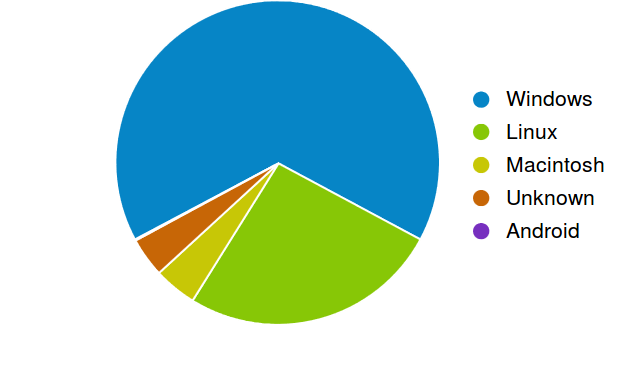
\includegraphics[width=\textwidth]{images/OTB4_download_sourceforge_os_crop.png}
\begin{center}
\tiny{Système d'exploitation des téléchargements sur Sourceforge (ne tient pas compte des autres dépôt)}
\end{center}
\end{columns}
\end{frame}

\begin{frame}
\frametitle{Flexibilité, passage à l'échelle: \textit{Pipeline}, \textit{Streaming} et \textit{multithreading}}

\begin{block}{Le modèle de \textit{Pipeline}}
\begin{center}
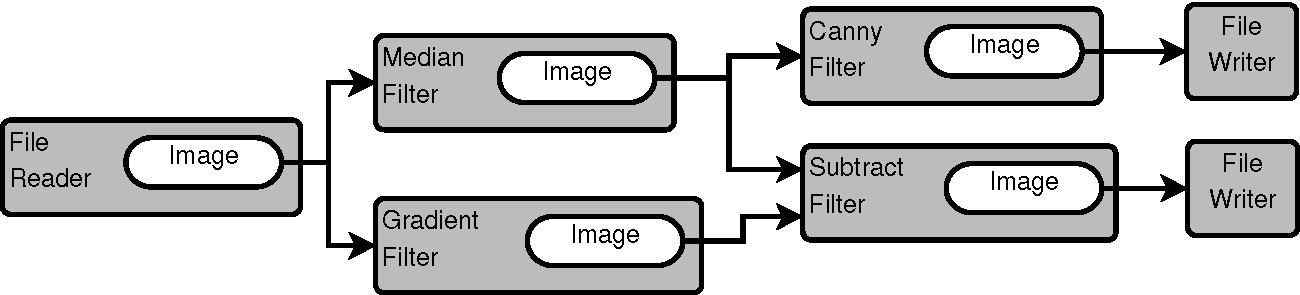
\includegraphics[width=0.7\textwidth]{images/ProcessObjectDataObject.png}
\end{center}
\end{block}
\vspace{-0.5cm}
\begin{block}{\textit{Streaming}}
\begin{center}
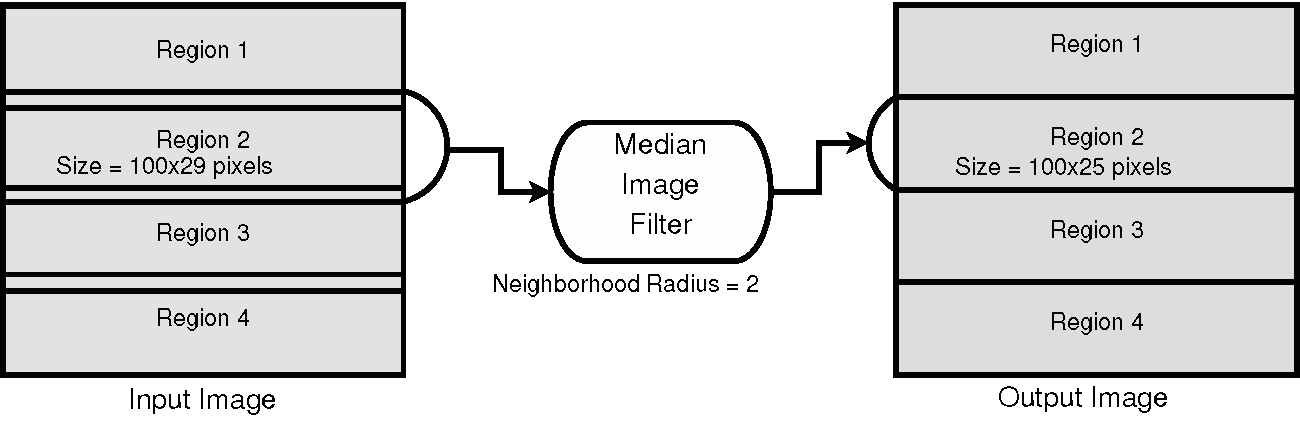
\includegraphics[width=0.7\textwidth]{images/StreamingImageDiagram.png}
\end{center}
\end{block}
\vspace{-0.5cm}
\begin{center}
\tiny{source: http://www.aosabook.org/en/itk.html}
\end{center}
\end{frame}

\begin{frame}
\frametitle{Flexibilité, passage à l'échelle: en coulisse ...}
\begin{center}
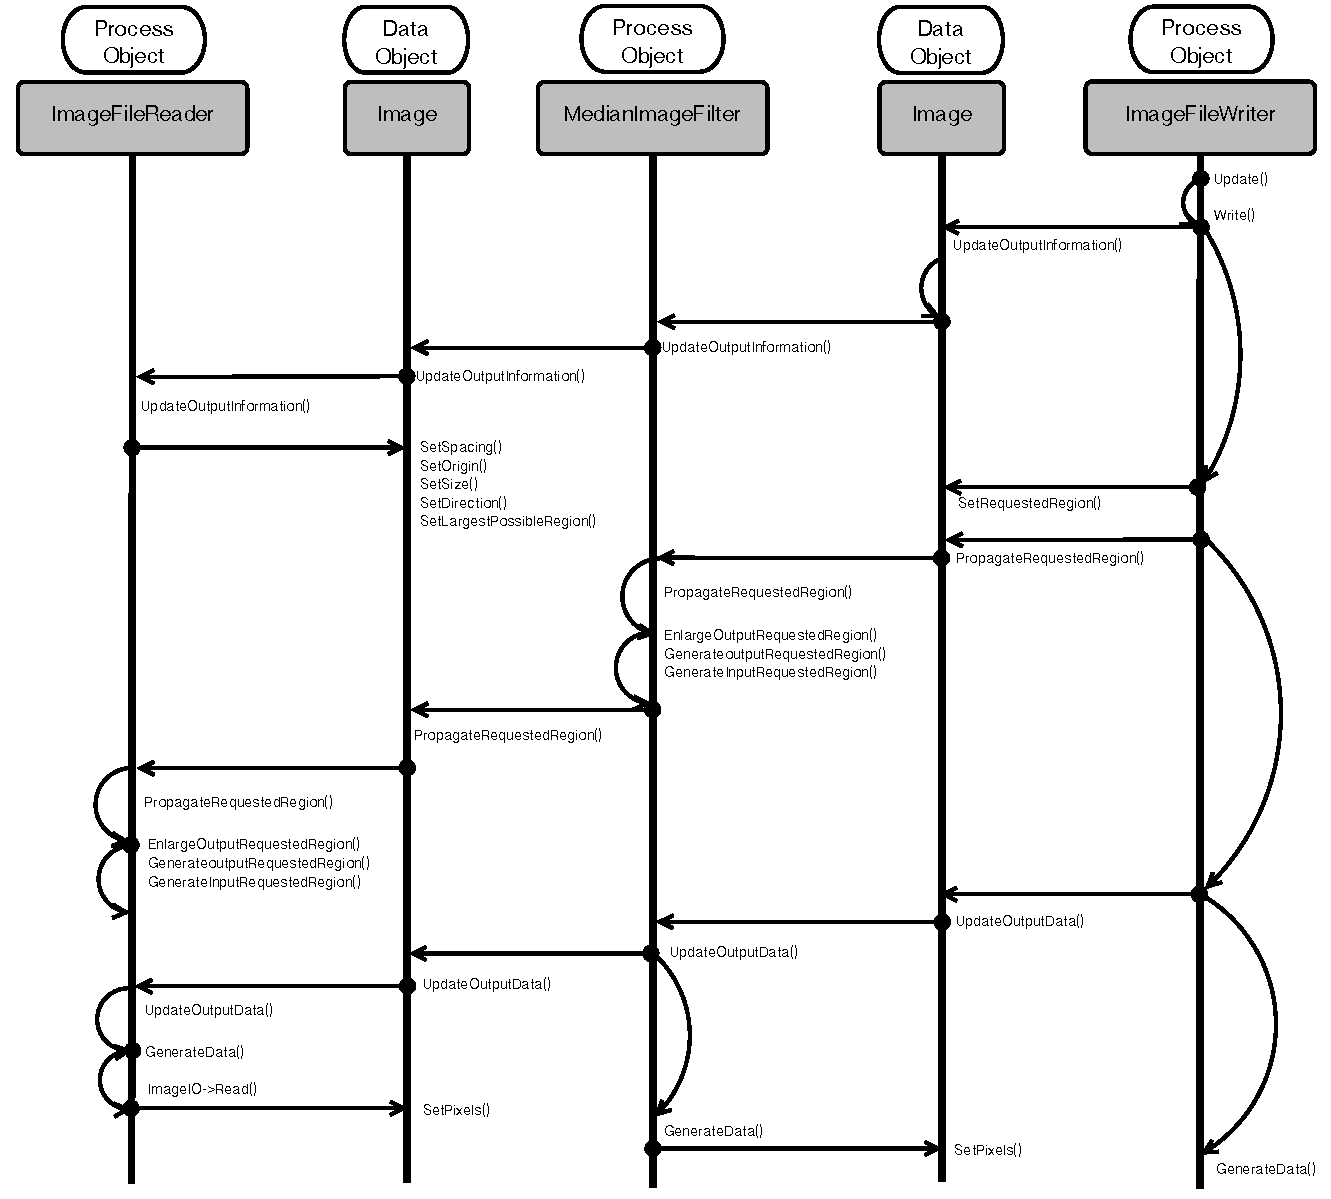
\includegraphics[width=0.6\textwidth]{images/ProcessObjectDataObjectInteractionUML.png}\\
\tiny{source: http://www.aosabook.org/en/itk.html}
\end{center}
\end{frame}

\begin{frame}
\frametitle{Proche de l'état de l'art}
\begin{itemize}
\item Veille technologique de l'équipe de développement
\item Implémentations d'algorithmes récents d'après publication. Ex.: profils morphologiques, segmentation MeanShift, textures de Haralick, points d'intérêt SURF \ldots
\item Implémentations de références contribuées par les auteurs de certains travaux en support à leur publication. Ex.: Large Scale MeanShift, fusion bayésienne, détection d'objets \ldots
\item Veille pour bénéficier des avancées des logiciels tiers. Ex.: algorithmes de \textit{machine learning} d'OpenCV,
\item Souvent: pour une même brique fonctionnelle, plusieurs algorithmes de complexités différentes disponibles sous une même interface.
\end{itemize}
\end{frame}


\begin{frame}
\frametitle{Un mot concernant le développement du logiciel}
\vspace{-0.5cm}
\begin{itemize}
\item Gestion de code source décentralisée: Git (migration depuis Mercurial en
  Juillet 2015)
\item C++ et suite CMake (CTest, CDash)
\item Développement guidé par les tests (TDD)
\item Gestion Agile (scrum)
\item Intégration continue et packaging automatisé
\end{itemize}
Tout les jours, environ 3000 tests sont compilés et rejoués sur 16
configurations différentes.
\begin{center}
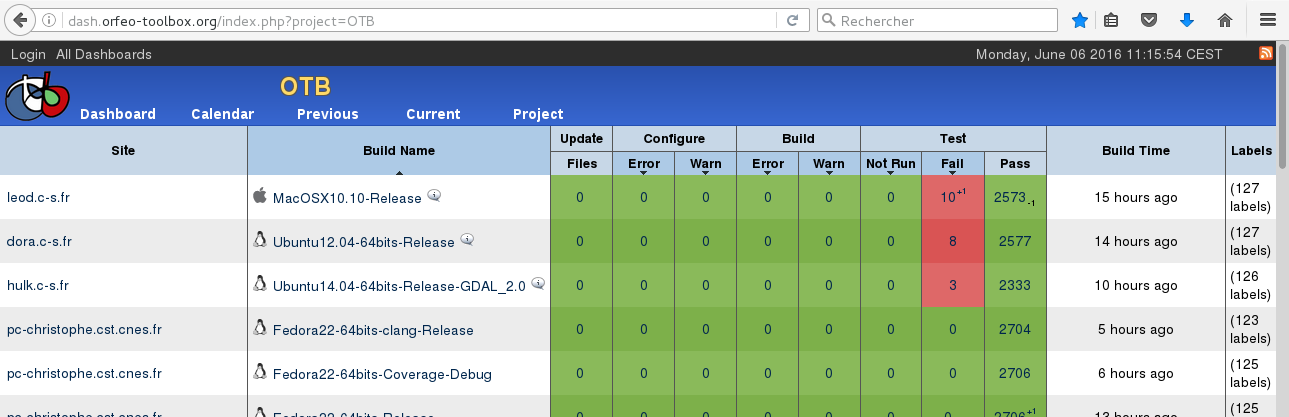
\includegraphics[width=\textwidth]{images/dashboard.png}
\end{center}
\end{frame}
